\chapter{Exercises}
\label{sec:15}
\abstract*{ In this chapter, we propose a series decision problems of various difficulties which may serve as exercises and exam questions for an Algorithmic Decision Theory or Multiple Criteria Decision Analysis course. They cover \emph{selection}, \emph{ranking} and \emph{rating} decision problems.}

\abstract{  In this chapter, we propose a series decision problems of various difficulties which may serve as exercises and exam questions for an Algorithmic Decision Theory or Multiple Criteria Decision Analysis course. They cover \emph{selection}, \emph{ranking} and \emph{rating} decision problems.}


\paragraph{Introduction}

The following exercises are marked as follows: \emph{warming up} (§), \emph{home work} (§§), \emph{research work} (§§§). Solutions should be supported both by computational Python code using the \Digraph programming resources as well as by methodological and algorithmic arguments from the \emph{Algorithmic Decision Theory} Lectures \citep{ADT-2020,BIS-2021b}.

\section{Who will receive the best student award? (§)}
\label{sec:15.1}

\paragraph{\textbf{Data}}

In Table~\vref{tab:15.1} you find the actual grades obtained by four students : \emph{Ariana} (\texttt{A}), \emph{Bruce} (\texttt{B}), \emph{Clare} (\texttt{C}) and \emph{Daniel} (\texttt{D}) in five courses: \texttt{C1}, \texttt{C2}, \texttt{C3}, \texttt{C4} and \texttt{C5} weighted by their respective \texttt{ECTS} points.\footnote{\texttt{ECTS} stands for \emph{European Credit Transfer System}. It is a unit used to grade diplomas in all participating countries \href{https://wwwen.uni.lu/studies/ects\_credits}{https://wwwen.uni.lu/studies/ects\_credits}}. 
\begin{table}[h]
\caption{Grades obtained by the students}
\label{tab:15.1}       % Give a unique label
\begin{center}
  %\begin{small}
    \begin{tabular}{l|c|c|c|c|c}
      \svhline\noalign{\smallskip}
      Course & \texttt{CF} & \texttt{C2} & \texttt{C3} & \texttt{C4} & \texttt{C5}\\
      \texttt{ECTS}   & 2  & 3  & 4  & 2  & 4\\
      \noalign{\smallskip}\hline\noalign{\smallskip}
      Ariana (\texttt{A})  &  11 & 13 &   9 & 15 &  11\\
      Bruce (\texttt{B})   & 12  & 9  &  13 & 10 &  13\\
      Clare (\texttt{C})   &   8 & 11 &  14 & 12 &  14\\
      Daniel (\texttt{D})  &  15 & 10 &  12 &  8 &  13\\
      \noalign{\smallskip}\hline
    \end{tabular}
  %\end{small}
\end{center}
\end{table}
The student grades are measured on an ordinal performance scale from $0$ pts (weakest) to $20$ pts (highest). Assume that the grading admits a preference discrimination threshold of $1$ point. No considerable performance differences are given. The more \texttt{ECTS} points, the more importance a course takes in the curriculum of the students. An award is to be granted to the student showing the \emph{best} result.

\paragraph{\textbf{Questions}}

\begin{enumerate}
\item Edit a \texttt{PerformanceTableau} instance with the data shown above (see Chapter~\ref{sec:5}). 
\item Who would you nominate for the grant?
\item Explain and motivate your selection algorithm.
\item Assume that the grading may actually admit an indifference discrimination threshold of $1$ point and a preference discrimination threshold of $2$ points. How stable is your grant recommendation with respect to this preference discrimination power of the grading scale?
\end{enumerate}

\section{How to fairly rank movies? (§)}
\label{sec:15.2}

\paragraph{\textbf{Data}}

File \texttt{graffiti03.py} \footnote{The file is provided in the \texttt{examples} directory of the \Digraph resources.} contains a performance tableau inspired by the star-rating of movies that could be seen in the city of Luxembourg during Spring 2003 (source: \citet{GRA-2003}). Its content is shown in Fig.~\vref{fig:15.1}.
\begin{lstlisting}
   >>> from perfTabs import PerformanceTableau
   >>> t = PerformanceTableau('graffiti03')
   >>> t.showHTMLPerformanceHeatmap(WithActionNames=True,\
   ...                        pageTitle='Graffiti Star wars',
   ...                        rankingRule=None,colorLevels=5,
   ...                        ndigits=0)   
\end{lstlisting}
\begin{figure}[ht]
%\sidecaption
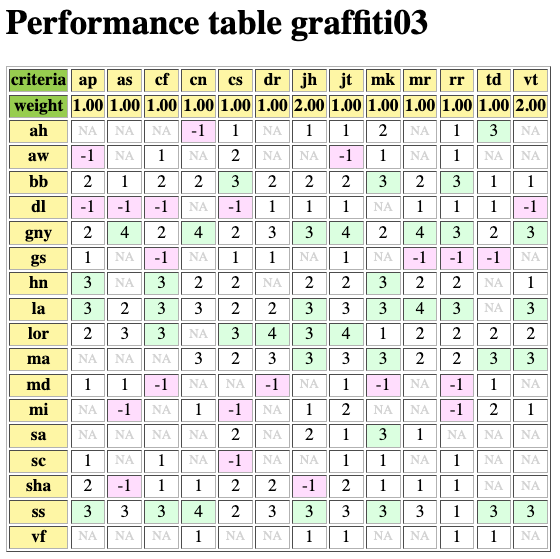
\includegraphics[width=0.9\hsize]{Figures/15-1-moviesRatingData.png}
\caption{Graffiti magazine's movie ratings from February 2003}
\label{fig:15.1}       % Give a unique label
\end{figure}

The critic's opinions are expressed on seven rating levels: $-2$ (two zeros, \emph{I hate}), $-1$ (one zero, \emph{I don't like}), $1$ (one star, \emph{maybe}), $2$ (two stars, \emph{good}), $3$ (three stars, \emph{excellent}), $4$ (four stars, \emph{not to be missed}), and $5$ (five stares, \emph{a master piece}). Notice the many missing data (\texttt{NA}) when a critic had not seen the respective movie. Mind also that the ratings of two movie critics (\texttt{jh} and \texttt{vt}) are given a higher significance weight.

\paragraph{\textbf{Questions}}

\begin{enumerate}
\item The \Graffiti magazine suggests a best rated movie by computing the average number of stars it received, ignoring the missing data and any significance weights of the critics. What movie gets the highest average? 
\item By taking into account missing data and varying significance weights, how may one find the best rated movie without computing any average of stars?
\item How would one rank these movies so as to at best respect the weighted rating opinions of each movie critic?
\item In what ranking position would appear a movie not seen by any critic? Confirm computationally your answer by adding such a fictive, \emph{not at all evaluated}, movie to the given performance tableau instance.
\item How robust are the preceding results when the significance weights of the movie critics are considered to be only ordinal grades?
\end{enumerate}

\section{What is your best choice recommendation? (§)}
\label{sec:15.3}


\paragraph{\textbf{Data}}

A person, who wants to buy a TV set, retains after a first selection, eight potential TV models \footnote{A similar didactic decision problem is discussed by \citet[pp.33-35]{VIN-1992}}. To make their best choice, these eight models were graded with respect to three decision objectives of equal importance:

\begin{enumerate}[topsep=3pt]
\item \emph{Costs} of the set (to be minimised); 
\item \emph{Picture and Sound} quality of the TV (to be maximised):
\item \emph{Maintenance contract} quality of the provider (to be maximised).
\end{enumerate}

The \emph{Costs} objective is assessed by the price of the TV set (criterion $Pr$ to be minimised). \emph{Picture} quality (criterion $Pq$), \emph{Sound} quality (criterion $Sq$) and \emph{Maintenance contract} quality (criterion $Mq$) are each one assessed on a four levels qualitative performance scale: -1 (\emph{not good}), 0 (\emph{average}), 1 (\emph{good}) and 2 (\emph{very good}).

The actual evaluation data are gathered in Table~\vref{tab:15.2}.
\begin{table}[h]
\caption{Performance evaluations of the potential TV sets}
\label{tab:15.2}       % Give a unique label
\begin{center}
  %\begin{small}
    \begin{tabular}{l|c|c|c|c}
      \svhline\noalign{\smallskip}
      Criteria & \texttt{Pr} (€) & \texttt{Pq} & \texttt{Sq} & \texttt{Mq} \\
      Significance & 2  & 1  & 1  & \\
      \noalign{\smallskip}\hline\noalign{\smallskip}
      Model \texttt{T1}   &     -1300  &  2  &  2  &   0\\
      Model \texttt{T2}   &     -1200  &  2  &  2  &   1\\
      Model \texttt{T3}   &     -1150  &  2  &  1  &   1\\
      Model \texttt{T4}   &     -1000  &  1  &  1  &  -1\\
      Model \texttt{T5}   &     -950   &  1  &  1  &   0\\
      Model \texttt{T6}   &     -950   &  0  &  1  &  -1\\
      Model \texttt{T7}   &     -900   &  1  &  0  &  -1\\
      Model \texttt{T8}   &     -900   &  0  &  0  &   0\\
      \noalign{\smallskip}\hline
    \end{tabular}
  %\end{small}
\end{center}
\end{table}

The \emph{Price} criterion \texttt{Pr} supports furthermore an indifference threshold of $25.00$€ and a preference threshold of $75.00$€. No considerable performance differences (veto thresholds) are to be considered.

\paragraph{\textbf{Questions}}

\begin{enumerate}
\item Edit a new \texttt{PerformanceTableau} instance with the data shown in Table~\vref{tab:15.2} and illustrate its content by best showing objectives, criteria, decision alternatives and performance table. If needed, write adequate python code.
\item What is the best TV set to recommend?
\item Illustrate your best choice recommendation with an adequate \emph{graphviz} drawing.
\item Explain and motivate your selection algorithm.
\item Assume that the qualitative criteria: \emph{Picture} quality (\texttt{Pq}), \emph{Sound} quality (\texttt{Sq}), and \emph{Maintenance contract} quality (\texttt{Mq}), are all three considered to be equi-significant and that the significance of the \emph{Price} criterion (\texttt{Pr}) equals the significance of these three quality criteria taken together. How stable is your best choice recommendation with respect to thus reviewing the criteria significance weights?
\end{enumerate}   

\section{What is the best public policy? (§§)}
\label{sec:15.4}

\paragraph{\textbf{Data files}}

\begin{itemize}
\item File \texttt{perfTab\_1.py} \footnote{Files \texttt{perfTab\_1.py} and \texttt{historicalData\_1.py} are provided in the \texttt{examples} directory of the \Digraph resources \citep{BIS-2021b}.} contains a 3-Objectives performance tableau with $100$ performance records concerning public policies evaluated with respect to an \emph{economic}, a \emph{societal} and an \emph{environmental} social decision objective.
\item File \texttt{historicalData\_1.py} contains a performance tableau of the same kind with $2000$ historical performance records.
\end{itemize}

\paragraph{\textbf{Questions}}

\begin{enumerate}
\item Illustrate the content of the given \texttt{perfTab\_1.py} performance tableau by best showing \emph{objectives}, \emph{criteria}, \emph{decision alternatives} (public policies) and \emph{performance evaluations}. If needed, write adequate python code.
\item Construct the corresponding bipolar-valued outranking digraph. How \emph{confident} and/or \emph{robust} are the apparent outranking situations?
\item What are apparently the $5$ best-ranked decision alternatives in your decision problem from the different decision objectives point of views and from a global fair compromise view? Justify your ranking approach from a methodological point of view.
\item How would you rate your 100 public policies into relative deciles classes?
\item Using the given historical records in file \texttt{historicalData\_1.py}, how would you rate your 100 public policies into absolute deciles classes? 
\item Explain the differences you may observe between the absolute and the previous relative rating result.
\item  Select among your 100 potential public policies a shortlist of up to 15 potential best policies, all reaching an absolute performance quantile of at least $66.67\%$.
\item Based on the previous best policies shortlist (see Question 6), what is your eventual best-choice recommendation? Is it perhaps a best choice unopposed by all three objectives?
\end{enumerate}

\section{A fair diploma validation decision (§§§)}
\label{sec:15.5}

\paragraph{\textbf{Data}}

Use the \texttt{RandomAcademicPerformanceTableau} class\index{RandomAcademicPerformanceTableau@\texttt{RandomAcademicPerformanceTableau} class} from the \texttt{random\-PerfTab} module for generating realistic random students performance tableaux concerning a curriculum of nine \texttt{ECTS} weighted Courses \citep{BIS-2021b}. Assume that all the gradings are done on an integer scale from $0$ (weakest) to $20$ (best). It is known that grading procedures are inevitably somehow imprecise; therefore assume an indifference discrimination threshold of $1$ point and a preference discrimination threshold of $2$ points. Furthermore, a performance difference of more than $12$ points is considerable and will trigger a polarisation situation. To validate eventually their curriculum, the students are required to obtain more or less $10$ points in each course. 

\paragraph{\textbf{Questions}}

\begin{enumerate}
\item Design and implement a fair diploma validation decision rule based on the grades obtained in the nine Courses.
\item Run simulation tests with random students performance tableaux for validating your design and implementation.
\end{enumerate}

%%%%%%% The chapter bibliography
%\normallatexbib
%\clearpage
%\phantomsection
%\addcontentsline{toc}{section}{Chapter Bibliography}
%\chapter{Exercises}
\label{sec:15}
\abstract*{We propose hereafter some decision problems which may serve as exercises and exam questions in an \emph{Algorithmic Decision Theory} Course. They cover \emph{selection}, \emph{ranking} and \emph{rating} decision problems.}

\abstract{We propose hereafter some decision problems which may serve as exercises and exam questions in an \emph{Algorithmic Decision Theory} Course. They cover \emph{selection}, \emph{ranking} and \emph{rating} decision problems.}

The exercises we propose in this Chapter are marked as follows: § (\emph{warming up}), §§ (\emph{home work}), §§§ (\emph{research work}). Solutions should be supported both by computational Python code using the \Digraph3 programming resources as well as by methodological and algorithmic arguments from the \emph{Algorithmic Decision Theory} Lectures [ADT-2020].

\section{Who will receive the best student award? (§)}
\label{sec:15.1}

\subsection{Data}
\label{sec:15.1.1}

Below in Table \ref{tab:15.1} you see the actual grades obtained by four students : \emph{Ariana} (A), \emph{Bruce} (B), \emph{Clare} (C) and \emph{Daniel} (D) in five courses: C1, C2, C3, C4 and C5 weighted by their respective ECTS points. 

\begin{table}[h]
\caption{Grades obtained by the students}
\label{tab:15.1}       % Give a unique label
\begin{center}
  %\begin{small}
    \begin{tabular}{l|c|c|c|c|c}
      \hline\noalign{\smallskip}
      Course & C1 & C2 & C3 & C4 & C5\\
      ECTS   & 2  & 3  & 4  & 2  & 4\\
      \noalign{\smallskip}\hline\noalign{\smallskip}
      Ariana (A)  &  11 & 13 &   9 & 15 &  11\\
      Bruce (B)   & 12  & 9  &  13 & 10 &  13\\
      Clare (C)   &   8 & 11 &  14 & 12 &  14\\
      Daniel (D)  &  15 & 10 &  12 &  8 &  13\\
      \noalign{\smallskip}\hline
    \end{tabular}
  %\end{small}
\end{center}
\end{table}

The grades shown in Table \ref{tab:15.1} are given on an ordinal performance scale from 0 pts (weakest) to 20 pts (highest). Assume that the grading admits a preference threshold of 1 points. No considerable performance differences are given. The more ECTS points, the more importance a course takes in the curriculum of the students. An award is to be granted to the \emph{best} amongst these four students.

\subsection{Questions}
\label{sec:15.1.2}

\begin{enumerate}
\item Edit a :ref:`PerformanceTableau <New-PerformanceTableau-Tutorial-label>` instance with the data shown above. 
\item Who would you nominate?
\item Explain and motivate your selection algorithm.
\item Assume that the grading may actually admit an indifference threshold of 1 point and a preference threshold of 2 points. How stable is your result with respect to the actual preference discrimination power of the grading scale?
\end{enumerate}

\section{How to fairly rank movies (§)}
\label{sec:15.2}

\subsection{Data}
\label{15.2.1}

- File \texttt{graffiti03.py}  contains a performance tableau about the rating of movies to be seen in the city of Luxembourg, February 2003. Its content is shown in Fig. \ref{fig:15.1} below.

\begin{lstlisting}
   >>> from perfTabs import PerformanceTableau
   >>> t = PerformanceTableau('graffiti03')
   >>> t.showHTMLPerformanceHeatmap(WithActionNames=True,\
   ...                        pageTitle='Graffiti Star wars',
   ...                        rankingRule=None,colorLevels=5,
   ...                        ndigits=0)   
\end{lstlisting}

\begin{figure}[h]
%\sidecaption
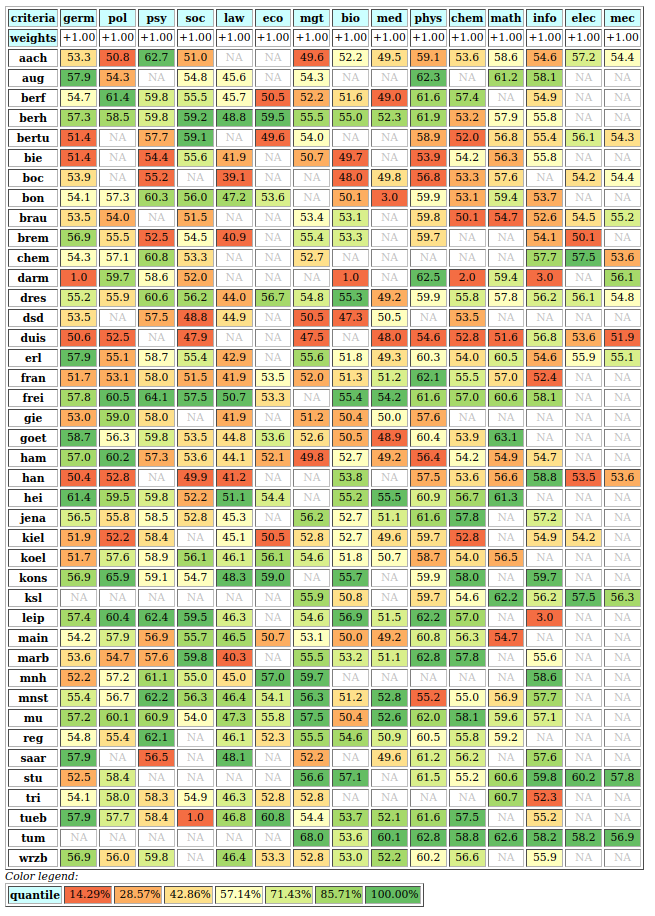
\includegraphics[width=10cm]{Figures/ratingData.png}
\caption{Graffiti magazine's movie ratings from February 2003}
\label{fig:15.1}       % Give a unique label
\end{figure}

The critic's opinions are expressed on a 7-graded scale: -2 (two zeros, \emph{I hate}), -1 (one zero, \emph{I don't like}), 1 (one star, \emph{maybe}), 2 (two stars, \emph{good}), 3 (three stars, \emph{excellent}), 4 (four stars, \emph{not to be missed}), and 5 (five stares, \emph{a master piece}). Notice the many missing data (\texttt{NA}) when a critic had not seen the respective movie. Mind also that the ratings of two movie critics ('jh' and 'vt') are given a higher significance weight.

\subsection{Questions}
\label{15.2.2}

\begin{enumerate}
\item The Graffiti magazine suggest a best rated movie with the help of an average number of stars, ignoring the missing data and any significance weights of the critics. By taking into account missing data and varying significance weights, how may one find the best rated movie without computing any average rating scores?
\item How would one rank these movies so as to at best respect the weighted rating opinions of each movie critic?
\item In what ranking position would appear a movie not seen by any movie critic? Confirm computationally the answer by adding such a fictive, \emph{not at all evaluated}, movie to the given performance tableau instance.
\item How robust are the preceeding results when the significance weights of the movie critics are considered to be only ordinal grades ?
\end{enumerate}

\section{What is your best choice recommendation? (§)}
\label{sec:15.3}


\subsection{Data}
\label{sec:15.3.1}

A person, who wants to by a TV set, retains after a first selection, eight potential TV models \footnote{The data is taken from Ph. Vincke, \emph{Multicriteria Decision-Aid}, John Wiley \& Sons Ltd, Chichester UK 1992, p.33-35.}. To make up her choice these eight models were evaluated with respect to three decision objectives of equal importance: - \emph{Costs} of the set (to be minimized); - \emph{Picture and Sound} quality of the TV (to be maximized): - \emph{Maintenace contract} quality of the provider (to be maximized).

The \emph{Costs} objective is assessed by the price of the TV set (criterion $Pr$ to be minimized). \emph{Picture} quality (criterion $Pq$), \emph{Sound} quality (criterion $Sq$) and \emph{Maintenace contract} quality (criterion $Mq$) are each one assessed on a four-level qualitative performance scale: -1 (\emph{not good}), 0 (\emph{average}), 1 (\emph{good}) and 2 (\emph{very good}).

The actual evaluation data are gathered in Table \ref{tab:15.2} below.    

\begin{table}[h]
\caption{Performance evaluations of the potential TV sets}
\label{tab:15.2}       % Give a unique label
\begin{center}
  %\begin{small}
    \begin{tabular}{l|c|c|c|c}
      \hline\noalign{\smallskip}
      Criteria & Pr (€) & Pq & Sq & Mq \\
      Significance & 2  & 1  & 1  & \\
      \noalign{\smallskip}\hline\noalign{\smallskip}
      Model T1   &     -1300  &  2  &  2  &   0\\
      Model T2   &     -1200  &  2  &  2  &   1\\
      Model T3   &     -1150  &  2  &  1  &   1\\
      Model T4   &     -1000  &  1  &  1  &  -1\\
      Model T5   &     -950   &  1  &  1  &   0\\
      Model T6   &     -950   &  0  &  1  &  -1\\
      Model T7   &     -900   &  1  &  0  &  -1\\
      Model T8   &     -900   &  0  &  0  &   0\\
      \noalign{\smallskip}\hline
    \end{tabular}
  %\end{small}
\end{center}
\end{table}

The \emph{Price} criterion 'Pr' supports furthermore an indifference threshold of $25.00$€ and a preference threshold of $75.00$€. No considerable performance differences (veto thresholds) are to be considered.

\subsection{Questions}
\label{sec:15.3.2}

\begin{enumerate}
\item Edit a new \texttt{PerformanceTableau} instance with the data shown above and illustrate its content by best showing objectives, criteria, decision alternatives and performance table. If needed, write adequate python code.
\item What is the best TV set to recommend?
\item Illustrate your best choice recommendation with an adequate \emph{graphviz} drawing.
\item Explain and motivate your selection algorithm.
\item Assume that the qualitative criteria: \emph{Picture} quality ('Pq'), \emph{Sound} quality ('Sq'), and \emph{Maintenace contract} quality ('Mq'), are all three considered to be equi-significant and that the significance of the \emph{Price} criterion ('Pr') equals the significance of these three quality criteria taken together. How stable is your best choice recommendation with respect to changing these criteria significance weights?
\end{enumerate}   

\section{What is the best public policy? (§§)}
\label{sec:15.4}

\subsection{Data files}
\label{sec:15.4.1}

\begin{itemize}
\item File \texttt{perfTab\_1.py} \footnote{The file \texttt{perfTab\_1.py} may be found in the \texttt{examples} directory of the \Digraph resources.} contains a 3 Objectives performance tableau with 100 performance records concerning public policies evaluated with respect to an \emph{economic}, a \emph{societal} and an \emph{environmental} public decision objective.
\item File \texttt{historicalData\_1.py} [footnote] contains a performance tableau of the same kind with 2000 historical performance records.
\end{itemize}

\subsection{Questions}
\label{sec:15.4.2}

\begin{enumerate}
\item Illustrate the content of the given file \texttt{perfTab\_1.py} performance tableau by best showing \emph{objectives}, \emph{criteria}, \emph{decision alternatives} and \emph{performance table}. If needed, write adequate python code.
\item Construct the corresponding bipolar-valued outranking digraph. How \emph{confident} and/or \emph{robust} are the apparent outranking situations?
\item What are apparently the 5 best-ranked decision alternatives in your decision problem from the different decision objectives point of views and from a global fair compromise view? Justify your ranking approach from a methodological point of view.
\item How would you rate your 100 public policies into relative deciles classes?
\item Using the given historical records in file \texttt{historicalData\_1.py}, how would you rate your 100 public policies into absolute deciles classes? Explain the differences you may observe between the absolute and the previous relative rating result.
\item  Select among your 100 potential policies a shortlist of up to 15 potential best policies,  all reaching an absolute performance quantile of at least $66.67\%$.
\item Based on the previous best policies shortlist (see Question 6), what is your eventual best-choice recommendation? Is it perhaps an unopposed best choice by all three objectives?
\end{enumerate}

\section{A fair diploma validation decision (§§§)}
\label{sec:15.5}

\subsection{Data}
\label{sec:15.5.1}

Use the \texttt{RandomAcademicPerformanceTableau} constructor from the \Digraph Python resources for generating realistic random students performance tableaux concerning a curriculum of nine ECTS weighted Courses. Assume that all the gradings are done on an integer scale from 0 (weakest) to 20 (best). It is known that all grading procedures are inevitably imprecise; therefore we will assume an indifference threshold of 1 point and a preference theshold of 2 points. Thurthermore, a performance difference of more than 12 points is considerable and will trigger a polarisation situation. To validate eventually their curriculum, the students are required to obtain more or less 10 points in each course. 

\subsection{Questions}
\label{sec:15.5.2}

\begin{enumerate}
\item Design and implement a fair diploma validation decision rule based on the grades obtained in the nine Courses.
\item Run simulation tests with random students performance tableaux for validating your design and implementation.
\end{enumerate}


\bibliographystyle{spbasic}
\bibliography{03-backMatters/reference}
